\section{Appendix}
% ****************

\subsection{Plotting with \texttt{matplotlib.pyplot}}
% ===================================================

The documentation of \texttt{matplotlib} and its modules is quite extensive
but it doesn't give a simple overview of how graphics are organized. Therefore this
section outlines the idea behind \texttt{pyplot} graphics and its components. 

\cmd{pyplot} is a layer on \texttt{matplotlib} to provide graphic facilities
similar to Matlab. \texttt{pyplot} appears to be the preferred way to plot
graphics in \texttt{python/matplotlib}. See also \href{http://matplotlib.org/faq/usage_faq.html}{matplotlib usage} and 
the tutorial \href{https://github.com/ericliang/matplotlib/blob/master/trunk/scipy06/oo_resources/leftwich_tut.txt}
{Getting Started With Matplotlib}.

So, first import the \cmd{pyplot} module:

\begin{verbatim}
import matplotlib.pyplot as plt
\end{verbatim}

and get some dummy data to play with:

\begin{verbatim}
import numpy as np

x= np.array([1, 2, 3, 4])
y= x**2
\end{verbatim}

Here \texttt{x} and \texttt{y} are numpy arrays, although \texttt{pyplot} accepts
any iterable.

\subsubsection{Figure}
% --------------------------
\begin{verbatim}
fig= plt.figure()
\end{verbatim}

\cmd{matplotlib.figure.Figure()} is the top level of a graphics where everything starts
and it is therefore the equivalent of a blank sheet of paper where you draw the plot on. Use \texttt{figure}
to set among other things the \textbf{size} of the figure (in inches) and the \textbf{dpi} resolution,
if applicable. More or less the call \texttt{fig= plt.figure()} is equivalent to
\texttt{R}'s \texttt{g<- ggplot()}. \texttt{figure()} can be called with only default parameters;
in fact, a call to \texttt{Figure} can be skipped altogheter (see below). 

\subsubsection{Axis}
% ------------------

\begin{verbatim}
axes= fig.add_subplot(1, 3, 2)
\end{verbatim}

To draw on a \texttt{Figure} object you need to put a set of \cmd{Axes} where you actually
draw stuff.

\texttt{Axes} can be put with \cmd{.add\_subplot} or \cmd{.add\_axes}. \texttt{add\_subplot}
is similar to \texttt{R} \texttt{par(mfrow= c(n, m))} in that it divides the figure
in \emph{n} rows and \emph{m} columns. The third argument in \texttt{add\_subplot} states
which subplot should be drawn upon. \emph{E.g.} \texttt{fig.add\_subplot(1, 3, 2)}
sets one row, three columns, and draws in the middle subplot (number 2).

Alternatively \cmd{.add\_axes} can be used to specify the characteristics of the
plotting box. It's roughly equivalent to \texttt{R} \texttt{par(mar= c(a, b, c, d))}
in that you set the position of the axes relative to the overall figure. It can also
be used to add plot on top of each other, like figure insets.

The \cmd{Axes} object can be used to control graphic parameters like x- and y-limits,
the axis labels and the plot title. It controls more or less what you can control with \texttt{R}'s \texttt{par()}.

As for \texttt{Figure}, you can add a subplot with only default arguments or skip
the call altogether.

\subsubsection{Plotting}
% ----------------------

\begin{verbatim}
axes.plot(x, y)
\end{verbatim}

Drawing is realized by adding stuff to the \texttt{Axes} object, typically by means
of \cmd{plot()} function. Similar to \texttt{R plot()}, with \texttt{plot} you can
set the plotting style (line, point), colour, etc. See \href{http://matplotlib.org/api/pyplot_api.html#matplotlib.pyplot.plot}
{pyplot.plot} for documentation of setting line styles and plotting features.

\subsubsection{Rendering}
% ----------------------

\begin{verbatim}
fig.savefig('filename.pdf')
fig.show()
plt.close()
\end{verbatim}

The actual plot is visualized with the \cmd{show()} method and saved to file with
\cmd{savefig()} method. By default, file format is deduced from file extension.
Finally, call \cmd{close} to close the grahic device(s).

\subsubsection{In practice...}
% ----------------------------

In practice you can take shortcuts to create plots. It is not strictly necessary
to explicitly set up a \texttt{Figure} and \texttt{Axes} object.

\begin{verbatim}
plt.plot(x, y, 'r--', lw= 2)
plt.plot(x, y, 'bo', markersize=12)
plt.xlabel('x-lab')
plt.xlim([0, 5])
plt.rc('font', size= 20)
plt.grid()
plt.savefig('figs/app_simple.pdf', bbox_inches= 'tight')
plt.show()
\end{verbatim}

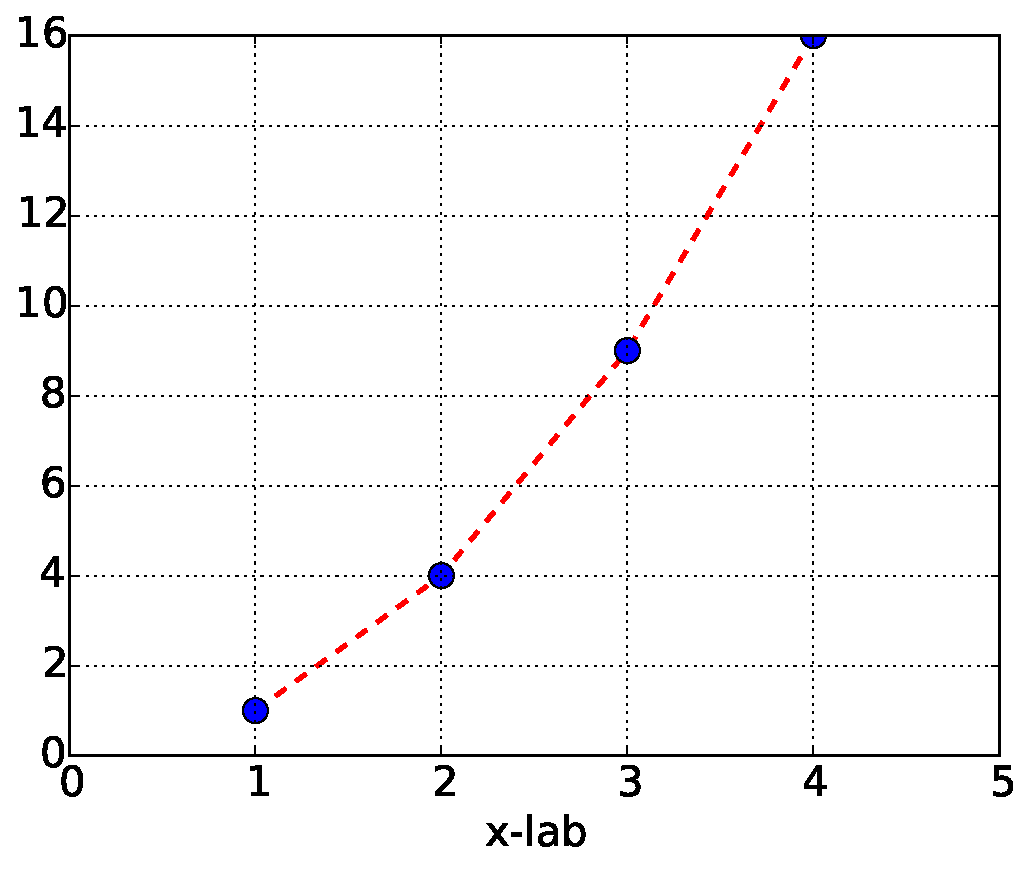
\includegraphics[width=0.5\linewidth]{figs/app_simple.pdf}

For simple plots, you can just call \cmd{plt.plot()} with the data to plot and
optional graphic paramaters. The bare minimum to see an xy-plot is just
\texttt{plt.plot(x, y); plt.show()}

Note that you keep adding features using \texttt{plt.<feature>},
then when you call \texttt{savefig} or \texttt{show} everything comes together.
In contrast to \texttt{R}, the order with which you add these features doesn't
matter. However, if you want to save to file \emph{and} show on screen, remember
to call \texttt{savefig} first and \texttt{show} then.

\begin{verbatim}
plt.rc('font', size= 8)
fig, axlst = plt.subplots(1, 3, sharex=True, sharey= True)
axlst[0].plot(x, y)
axlst[1].plot(x, y*2)
axlst[2].plot(x, y*3)
fig.subplots_adjust(wspace= 0.1)
fig.set_size_inches(18/2.54, 6/2.54)
fig.savefig('figs/app_subplot.pdf')
fig.show()
\end{verbatim}

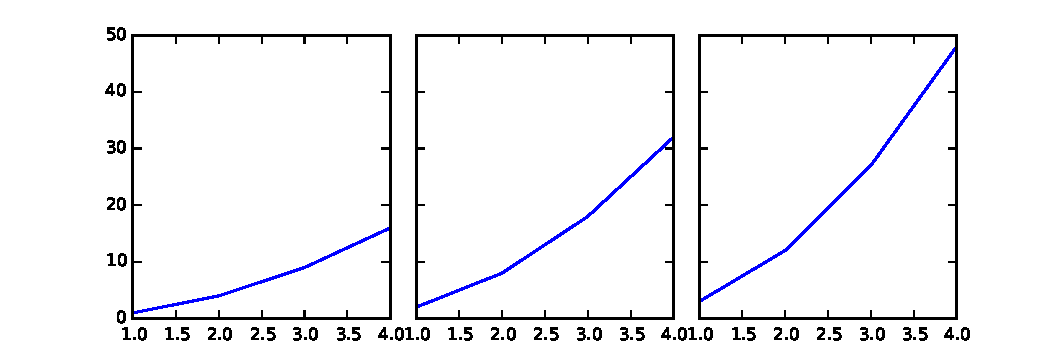
\includegraphics[width=\linewidth]{figs/app_subplot.pdf}

For multiple plots it might be best to set up the \texttt{Figure} object and the
list (array actually) of subplots in one call to \cmd{plt.subplots()}. Each element
of the array contains an \texttt{Axes} object that can be individually populated.
The \texttt{Axes}'s can be juxtaposed by playing with the method \cmd{Figure.subplots\_adjust}.
For example to set the spacing. 

\subsubsection{Example}
% ---------------------

\begin{verbatim}

fig= plt.figure()
ax1= fig.add_subplot(1, 3, 1)
ax1.plot(x, y, 'r--')
ax2= fig.add_subplot(1, 3, 2)
ax2.plot(x, y, 'pg')
ax3= fig.add_subplot(1, 3, 3)
ax3.plot(x, y, 'p')
for i, txt in enumerate(x):
    ax3.annotate(txt, (x[i], y[i]))
fig.show()
\end{verbatim}

\subsection{Principal components}
% ===============================

\dots

For interpretation of eigenvalues and eigenvectors of a covariance matrix see
http://www.visiondummy.com/2014/04/geometric-interpretation-covariance-matrix/

\subsection{PageRank}
% ===================

Google ranks pages predominantly according to two criteria: 1) Number of links a page
receives, \emph{i.e.} many other pages rerfers to it, or in other words it is 'cited' very often;
2) Incoming links are not all equal, incoming links from important pages are more
important, \emph{i.e.} being 'cited' by a very important page counts more.

See also \href{http://www.math.cornell.edu/~mec/Winter2009/RalucaRemus/Lecture3/lecture3.html}{The Mathematics of Google Search}

Stochastic matrix, \textit{i.e.} where column sums equal 1, describing how node weights
are distibuted.

\begin{equation}
\mathbf{A} = \left[\begin{matrix}0 & 0 & 1.0 & 0.5\\0.3 & 0 & 0 & 0\\0.3 & 0.5 & 0 & 0.5\\0.3 & 0.5 & 0 & 0\end{matrix}\right]
\end{equation}

\begin{itemize}
\item Each \textbf{column} describes how each node distributes its weight.

For example, $1^{st}$ column, $[0\ \frac{1}{3}\ \frac{1}{3}\ \frac{1}{3}]^T$, says that node $x_1$ gives 0 of its
weight to itself (of course), 1/3 to $x_2$, 1/3 to $x_3$, and 1/3 to $x_4$;
$4^{th}$ column describes node $x_4$ and it says that 1/2 weight is given to $x_1$,
0 to $x_2$, 1/2 to $x_3$, and 0 to itself.

\item Each \textbf{row} describes the weight or score of each node, since it is the SUM
of all the node weights.

For example, $1st$ row is the score for node $x_1$. $x_1$
receives 0 from itself (of course), 0 of the weight of $x_2$, 1 (\textit{i.e. all})
of the weight from $x_3$, and 1/2 of the weight from $x_4$.
\end{itemize}

So matrix \textbf{A} tells the \textit{proportion} of weight to and from nodes. The question
is: \emph{How much each node weighs?} If all the nodes had the same weight the row sums
of \textbf{A} would give the page rank already. However, we want to give more weight
to pages that have many incoming links and/or incoming links from high ranking pages.
For example, node $x_1$ receives all of the weight from $x_3$ (1) and half of the weight
from $x_4$ (0.5). But how much do $x_3$ and $x_4$ weigh?

The assign weights to nodes we need to solve the linear system where the LHS is
matrix \textbf{A} and RHS is the vector of weights (ranks) we want to find out:

\begin{equation}
\left[\begin{matrix}
0 x_1 + 0 x_2 + 1 x_{3} + 0.5 x_{4} \\
0.3 x_{1}  + 0 x_2 + 0 x_3 + 0 x_4 \\
0.3 x_{1} + 0.5 x_{2} + 0 x_3 + 0.5 x_{4} \\
0.3 x_{1} + 0.5 x_{2} + 0 x_3 + 0 x_4
\end{matrix}\right] =
\left[\begin{matrix}x_{1}\\ x_{2}\\x_{3}\\x_{4}\end{matrix}\right]
\end{equation}

This is equivalent to finding the eigenvector of \textbf{A} for the eigenvalue 1.
In fact see that if we set $\left[\begin{matrix}x_{1}\\x_{2}\\x_{3}\\x_{4}\end{matrix}\right] = \mathbf{u}$,
we have in matrix notation:

\begin{equation}
\mathbf{Au = \lambda u}; \quad and\ for\ \lambda = 1: \quad \mathbf{Au = u}; 
\end{equation}

which is the definition of eigenvectors/values. Note that since \textbf{A} is
stochastic the largest eigenvalue is always 1 \footnote{see also
\href{http://math.stackexchange.com/questions/40320/proof-that-the-largest-eigenvalue-of-a-stochastic-matrix-is-1}
{proof that the largest eigenvalue of a stochastic matrix} on Math Stack Exchange.}.

In this example the eigenvector for $\lambda = 1$ is $\mathbf{u} = \left[\begin{matrix}1\\0.33\\0.75\\0.5\end{matrix}\right]$.
We can normalize the scores to sum to 1 and obtain the pageRank
$PR =
\left[\begin{matrix}x_{1}\\x_{2}\\x_{3}\\x_{4}\end{matrix}\right] =
\left[\begin{matrix}0.39\\0.13\\0.29\\0.19\end{matrix}\right]$

Represent the web as a grpah and implement it as a dictionary of dictionaries. The outer dictionary has pages
(nodes) as keys. The value of each key (page) is a dictionary of outgoing links.
This inner dictionary has key: The arraival page, value: The weight transferred to
that page.

\begin{verbatim}
graph= {
    1: {2: 0, 3: 0, 4: 0},
    2: {3: 0, 4: 0},
    3: {1: 0},
    4: {1: 0, 3: 0}
}

# Assign weights to pages. Outgoing links:
for p in graph:
    pout= graph[p]
    for w in pout:
        pout[w]= 1.0 / len(pout)

# Matrix representation
pages= sorted(graph.keys())
A= np.array(zeros(len(pages), len(pages)))
for ci in range(len(pages)):
    page= graph[pages[ci]]
    for ri in range(len(pages)):
        outk= pages[ri]
        if outk in page:
            A[ri][ci]= page[outk]
A= Matrix(A)

# Solve A * u = u in order to get the ranks u:
u= Matrix(symbols('x1:%s' %(A.cols+1)))
Au= Eq(A*u, u)
sols= solve(Au.subs(x1, 1), u[1:])
sols[x1]= 1

# Or get all eigenvects, but slower since it calculates all of them:
A.eigenvects()[0]

# Normalize ranks to sum to 1
s= sum(sols.values())
pageRank= {}
for x in sols:
    pageRank[x]= sols[x]/s

PR= Matrix([pageRank[x] for x in u])

# Test we did it right
Eq(A * PR, PR) # True

\end{verbatim}

What if a page has no outgoing links? For example
\footnote{From J. Hefferon - Linear Algebra, Topic: Page Ranking}, in this graph
page 4 has no outgoing links:

\begin{verbatim}
graph= {
    1: {2:0},
    2: {3: 0},
    3: {1: 0, 2: 0, 4: 0},
    4: {}
}
\end{verbatim}

In this case we can imaging that a surfer reaching page 4 will move at random to
any other page. \emph{I.e.} we distribute the weight of page 4 uniformaly across
all the other pages:

\begin{verbatim}
for p in graph:
    pout= graph[p]
    if pout == {}:
        # If a page has no outgoing links distribute its weight across all web 
        for x in graph:
            graph[p][x]= 1.0 / len(graph)
    else:
        for w in pout:
            pout[w]= 1.0 / len(pout)
        graph[p]= pout
\end{verbatim}

This web looks like:

\begin{verbatim}
graph= 
{1: {2: 1.0},
 2: {3: 1.0},
 3: {1: 0.33, 2: 0.33, 4: 0.33},
 4: {1: 0.25, 2: 0.25, 3: 0.25, 4: 0.25}}
\end{verbatim}

As above, transform the graph in a stochastic matrix:

$$
\mathbf{A} = \left[\begin{matrix}0 & 0 & 0.33 & 0.25\\1.0 & 0 & 0.33 & 0.25\\0 & 1.0 & 0 & 0.25\\0 & 0 & 0.33 & 0.25\end{matrix}\right]
$$

\begin{verbatim}
pages= sorted(graph.keys())
A= np.array(zeros(len(pages), len(pages)))
for ci in range(len(pages)):
    page= graph[pages[ci]]
    for ri in range(len(pages)):
        outk= pages[ri]
        if outk in page:
            A[ri][ci]= page[outk]
A= Matrix(A)
\end{verbatim}

Obtain eigenvector for $\lambda= 1$ and normalize to have ranks to sum to 1
$$
PR = \left[\begin{matrix}0.16\\0.32\\0.36\\0.16\end{matrix}\right]
$$

Remember that there is an infinite number of eigenvectors belonging to an eigenvalue.
In fact we talk about \emph{eigenspace}. For convenience we choose the eigenvector
whose sum is 1.

\begin{verbatim}
def rankMatrix(A):
    """Return page ranks for matrix of weights A"""
    u= Matrix(symbols('x1:%s' %(A.cols+1)))
    Au= Eq(A*u, u)
    Au= Au.subs(x1, 1) # This sub is arbitrary, any real will do.
    sols= solve(Au, u[1:])
    sols[x1]= 1
    
    s= sum(sols.values())
    pageRank= {}
    for x in sols:
        pageRank[x]= sols[x]/s
    PR= Matrix([pageRank[x] for x in u])
    return PR
\end{verbatim}

Google edits the page rank matrix \textbf{A} to add some randomess in the behaviour
of the surfer. That is, a surfer every now and then might jump to a page not linked
in to the current one. The probability of jumping to an unlinked page is $\alpha$,
typically between 0.85 and 0.99.
To model this behaviour we edit the weight matrix \textbf{A} as follow:

\begin{itemize}
\item Edit the weights in weight matrix \textbf{A} by multiplying by the correction
factor $\alpha$, $\mathbf{A_{rnd}} = \alpha \mathbf{A}$.

\item Add to the corrected matrix $\alpha\mathbf{A}$ weights so that it returns to
be stochastic, \emph{i.e.} add $(1 - \alpha) \mathbf{R}$ where \textbf{R} is a matrix
of the same dim as \textbf{A} and with column sums 1.
\end{itemize}

Putting it all together, we obtain the \emph{Google matrix} \textbf{G} with the \emph{linear
combination}:

$$
\mathbf{G} = \alpha \mathbf{A} + (1 - \alpha) \mathbf{R}
$$

For this example:

$$
\mathbf{G} =
\alpha \left[\begin{matrix}0 & 0 & 0.33 & 0.25\\1.0 & 0 & 0.33 & 0.25\\0 & 1.0 & 0 & 0.25\\0 & 0 & 0.33 & 0.25\end{matrix}\right] +
(1 - \alpha) \left[\begin{matrix}0.25 & 0.25 & 0.25 & 0.25\\0.25 & 0.25 & 0.25 & 0.25\\0.25 & 0.25 & 0.25 & 0.25\\0.25 & 0.25 & 0.25 & 0.25\end{matrix}\right] =
$$

$$
\left[\begin{matrix}0 & 0 & 0.28 & 0.2125\\0.85 & 0 & 0.28 & 0.2125\\0 & 0.85 & 0 & 0.2125\\0 & 0 & 0.28 & 0.2125\end{matrix}\right] +
\left[\begin{matrix}0.0375 & 0.0375 & 0.0375 & 0.0375\\0.0375 & 0.0375 & 0.0375 & 0.0375\\0.0375 & 0.0375 & 0.0375 & 0.0375\\0.0375 & 0.0375 & 0.0375 & 0.0375\end{matrix}\right] =
\left[\begin{matrix}0.0375 & 0.0375 & 0.32 & 0.25\\0.8875 & 0.0375 & 0.32 & 0.25\\0.0375 & 0.8875 & 0.0375 & 0.25\\0.0375 & 0.0375 & 0.32 & 0.25\end{matrix}\right]
$$

The page ranks now become $PR_{\alpha=0.85} = \left[\begin{matrix}0.17 \\0.36 \\0.34 \\0.17 \end{matrix}\right]$.

Note that if $\alpha = 1$ than there is no randomess at all. If $\alpha = 0$ instead
the surfing is complete random and the page ranks become $PR_{\alpha=1} = \left[\begin{matrix}0.25\\0.25\\0.25\\0.25\end{matrix}\right]$

\begin{verbatim}
def googleRank(A, alpha= 0.85):
    """Ranks pages in weight matrix A after having add some random surfing
    behaviour alpha"""
    R= Matrix(A.rows, A.cols, [1/A.cols] * A.rows * A.cols)
    G = alpha * A + (1 - alpha) * R
    PR= rankMatrix(G)
    return PR

googleRank(A, 0.85)
\end{verbatim}

\subsection{Line of best fit (least squares)}
% ===========================================

\dots
